\documentclass[11pt]{article}

%% MinionPro fonts 
%\usepackage[lf]{MinionPro}
%\usepackage{MnSymbol}
\usepackage{microtype}

%% Margins
\usepackage{geometry}
\geometry{verbose,letterpaper,tmargin=1in,bmargin=1in,lmargin=1in,rmargin=1in}

%% Other packages
\usepackage{amsmath}
\usepackage{amsthm}
\usepackage{amsfonts}
\usepackage[shortlabels]{enumitem}
\usepackage{titlesec}
\usepackage{soul}
\usepackage{tikz}
\usepackage{mathtools}
\usepackage{pgfplots}
\usepackage{tikz-3dplot}
\usepackage{algorithmic}
\usepackage[export]{adjustbox}
\usepackage{tcolorbox}
\usepackage{mathrsfs}
\usepackage{multicol}
\usepackage{framed}
%\usepackage{optprog}


%% Paragraph style settings
\setlength{\parskip}{\medskipamount}
\setlength{\parindent}{0pt}

%% Change itemize bullets
\renewcommand{\labelitemi}{$\bullet$}
\renewcommand{\labelitemii}{$\circ$}
\renewcommand{\labelitemiii}{$\diamond$}
\renewcommand{\labelitemiv}{$\cdot$}

%% Colors
\definecolor{rred}{RGB}{204,0,0}
\definecolor{ggreen}{RGB}{0,145,0}
\definecolor{yyellow}{RGB}{255,185,0}
\definecolor{bblue}{rgb}{0.2,0.2,0.7}
\definecolor{ggray}{RGB}{190,190,190}
\definecolor{ppurple}{RGB}{160,32,240}
\definecolor{oorange}{RGB}{255,165,0}

%% Shrink section fonts
\titleformat*{\section}{\normalsize\bf}
\titleformat*{\subsection}{\normalsize\bf}
\titleformat*{\subsubsection}{\normalsize\it}

% %% Compress the spacing around section titles
\titlespacing*{\section}{0pt}{1.5ex}{0.75ex}
\titlespacing*{\subsection}{0pt}{1ex}{0.5ex}
\titlespacing*{\subsubsection}{0pt}{1ex}{0.5ex}

%% amsthm settings
\theoremstyle{definition}
\newtheorem{problem}{Problem}
\newtheorem{example}{Example}
\newtheorem*{theorem}{Theorem}
\newtheorem*{bigthm}{Big Theorem}
\newtheorem*{biggerthm}{Bigger Theorem}
\newtheorem*{bigcor1}{Big Corollary 1}
\newtheorem*{bigcor2}{Big Corollary 2}

%% tikz settings
\usetikzlibrary{calc}
\usetikzlibrary{patterns}
\usetikzlibrary{decorations}
\usepgfplotslibrary{polar}

%% algorithmic setup
\algsetup{linenodelimiter=}
\renewcommand{\algorithmiccomment}[1]{\quad// #1}
\renewcommand{\algorithmicrequire}{\emph{Input:}}
\renewcommand{\algorithmicensure}{\emph{Output:}}

%% Answer box macros
%% \answerbox{alignment}{width}{height}
\newcommand{\answerbox}[3]{%
  \fbox{%
    \begin{minipage}[#1]{#2}
      \hfill\vspace{#3}
    \end{minipage}
  }
}

%% \answerboxfull{alignment}{height}
\newcommand{\answerboxfull}[2]{%
  \answerbox{#1}{6.38in}{#2} 
}

%% \answerboxone{alignment}{height} -- for first-level bullet
\newcommand{\answerboxone}[2]{%
  \answerbox{#1}{6.0in}{#2} 
}

%% \answerboxtwo{alignment}{height} -- for second-level bullet
\newcommand{\answerboxtwo}[2]{%
  \answerbox{#1}{5.8in}{#2}
}

%% special boxes
\newcommand{\wordbox}{\answerbox{c}{1.2in}{.7cm}}
\newcommand{\catbox}{\answerbox{c}{.5in}{.7cm}}
\newcommand{\letterbox}{\answerbox{c}{.7cm}{.7cm}}

%% Miscellaneous macros
\newcommand{\tstack}[1]{\begin{multlined}[t] #1 \end{multlined}}
\newcommand{\cstack}[1]{\begin{multlined}[c] #1 \end{multlined}}
\newcommand{\ccite}[1]{\only<presentation>{{\scriptsize\color{gray} #1}}\only<article>{{\small [#1]}}}
\newcommand{\grad}{\nabla}
\newcommand{\ra}{\ensuremath{\rightarrow}~}
\newcommand{\maximize}{\text{maximize}}
\newcommand{\minimize}{\text{minimize}}
\newcommand{\subjectto}{\text{subject to}}
\newcommand{\trans}{\mathsf{T}}
\newcommand{\bb}{\mathbf{b}}
\newcommand{\bx}{\mathbf{x}}
\newcommand{\bc}{\mathbf{c}}
\newcommand{\bd}{\mathbf{d}}

%% LP format
%    \begin{align*}
%      \maximize \quad & \mathbf{c}^{\trans} \mathbf{x}\\
%      \subjectto \quad & A \mathbf{x} = \mathbf{b}\\
%                       & \mathbf{x} \ge \mathbf{0}
%    \end{align*}

%Space between rows:
%\def\arraystretch{2.2}
%
%Space between columns:
%\arraycolsep=1.4pt


%% Redefine maketitle
\makeatletter
\renewcommand{\maketitle}{
  \noindent SA405 -- AMP \hfill Rader \S 13.1  \\

  \begin{center}\Large{\textbf{\@title}}\end{center}
}
\makeatother

%% ----- Begin document ----- %%
\begin{document}
  
\title{Lesson 15.  IP Formulations, Part 1}

\maketitle

%%%
\section{Today}
\renewcommand\labelitemi{--}
\begin{itemize}
\item  LP review
\item  IP formulations
\end{itemize}

\section{Solving Integer Programs can be \emph{Really} Hard!}

The following integer (linear) program (IP) seeks an objective-maximizing integer linear combination of a big number. 
\begin{align*}
      \maximize \quad & 213x_1 - 1928x_2 - 11111x_3 - 2345x_4 + 9123x_5
\\
      \subjectto \quad & 12223x_1 + 12224x_2 + 36674x_3 + 61119x_4 + 85569x_5 = 89643482\\
                       & x_1,~x_2,~x_3,~x_4,~x_5 \ge 0, \text{ integer }
\end{align*}

\begin{problem}
We will solve two versions of the problem above.  
In both cases, use the \texttt{tee=True} flag to see the solver output in Jupyter as follows:

\vspace{-.5cm}
\begin{verbatim}
       solver_result = pyo.SolverFactory(`glpk').solve(model, tee=True)
\end{verbatim}

\begin{enumerate}[(a)]
\item  First solve the \textbf{LP relaxation} of the IP, which means allowing the variables to be continuous rather than integer-valued:  \texttt{domain=pyo.NonNegativeReals}

Does the solver arrive at an optimal solution? If so, list it here.  If not, what happens? \\ 
\answerboxone{c}{.5in}
\item Now solve the IP as written, which means requiring the variables to take integer values:  \texttt{domain=pyo.NonNegativeIntegers}

Does the solver arrive at an optimal solution? If so, list it here.  If not, what happens? \\ 
\answerboxone{c}{.5in}
\end{enumerate}
\end{problem}

\begin{tcolorbox}
In general, \catbox s are much harder to solve than \catbox s.
\end{tcolorbox}

\renewcommand\labelitemi{$\bullet$}
\begin{itemize}
\item This week we will discuss why this is, and why the way we model IP problems (yes, there are choices!) can impact solver performance.
\item Next week, we will learn about the \textbf{branch and bound algorithm} (B\&B), which is used by most IP solvers.  It is significantly more computationally-expensive than the LP simplex method.
\end{itemize}

\section{LP Review}

\begin{problem}  
Solve the following LP graphically: Shade the feasible region, draw two objective contours:  $x_1 +x_2 =2$ and $x_1 + x_2 =4$.  Use arrows to indicate the direction of an increasing objective value.  Label the optimal solution.  

\begin{minipage}{0.6\textwidth}
$
\begin{array}{rl}
\text{max} & x_1+x_2 \\
\text{s.t.} & x_1+2x_2 \leq 10 \\
  & x_1  \leq  4 \\
  & x_1, x_2  \geq  0
\end{array}
$

\bigskip
What is the optimal objective value?
 \catbox
\end{minipage}
\begin{minipage}{0.4\textwidth}
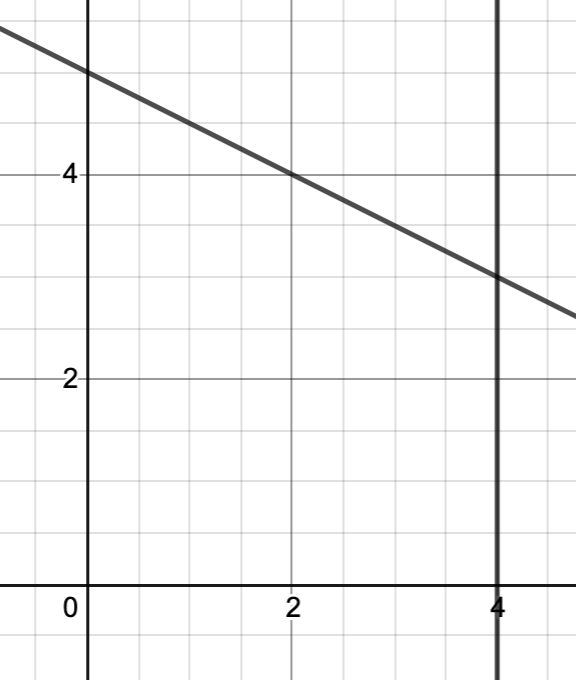
\includegraphics[width=0.7\textwidth]{LP_graph}
\end{minipage}



\end{problem}
\bigskip

\begin{tcolorbox}
\textbf{Theorem:} Every linear program (LP) has EXACTLY ONE of the following outcomes: 

\medskip
\begin{tabular}{ll}
(1) Unique optimal solution  ~~~~~& (3) Unbounded    \\
(2) Multiple optimal solutions & (4) Infeasible
\end{tabular}
\end{tcolorbox}

\begin{problem}
Sketch graphs that illustrate each of the  LP outcomes.
\end{problem}

\answerbox{c}{.5\textwidth}{2in} \answerbox{c}{.5\textwidth}{2in}

\answerbox{c}{.5\textwidth}{2in} \answerbox{c}{.5\textwidth}{2in}


\begin{tcolorbox}
\textbf{Theorem:}  Integer programs (IPs) have the same four possible outcomes as LPs: 

\medskip
\begin{tabular}{ll}
(1) Unique optimal solution  ~~~~~& (3) Unbounded    \\
(2) Multiple optimal solutions & (4) Infeasible
\end{tabular}

\end{tcolorbox}
\begin{tcolorbox}
\textbf{Theorem:} If an LP has an optimal solution (the LP is not unbounded or infeasible), an optimal solution can always be found at a 
\wordbox \wordbox %\textbf{corner point} 
of the feasible region.
\end{tcolorbox}

\textbf{Question:}  Is the same true for IPs?  In other words, if an optimal solution to an IP exists, can an optimal solution always be found at a corner point?  
\begin{itemize}
\item Keep this question in mind.  We will revisit it a little later.
\end{itemize}

\vfill

\section{IP Formulations}

\begin{tcolorbox}
A \textbf{formulation} of an IP is a set of linear \wordbox that capture ALL of the \wordbox integer points, and NO OTHER integer points.
\end{tcolorbox}

\begin{itemize}
\item  We will see some examples of formulations of an IP in the next problem.
\end{itemize}

\bigskip
\begin{tcolorbox}
The \textbf{LP relaxation} of an IP is the LP that is formed by \emph{relaxing} the integer requirement on the variables.
\end{tcolorbox}

%\textbf{Question:} What makes \emph{integer} linear programs so much harder to solve than \emph{continuous} linear programs?  
%
%\bigskip
%\textbf{Answer:}  Because if we require our solution to be integer-valued the optimal solution doesn't usually occur at a \wordbox \wordbox of the feasible region!  (We will see this graphically.) 
%
%
%\bigskip
%This makes the \textbf{formulation} or \textbf{modeling}, of integer programs incredibly important.



\newpage
\begin{problem}  
Below are two integer programs, along with the diagrams of their constraints. (Rader, examples 13.3, 13.4) 

\begin{multicols}{2}

{\bf Problem A:}
\begin{align*}
      \maximize \quad & 8x + 7y \\
      \subjectto \quad & -18x + 38y ~~\leq~~ 133\\
                       & 13x + 11y ~\leq~ 125\\
                       & 10x - 8y ~\leq~ 55\\
                       & x,y \in \mathbb{Z}^{\geq 0}
\end{align*}
\vspace{6cm}

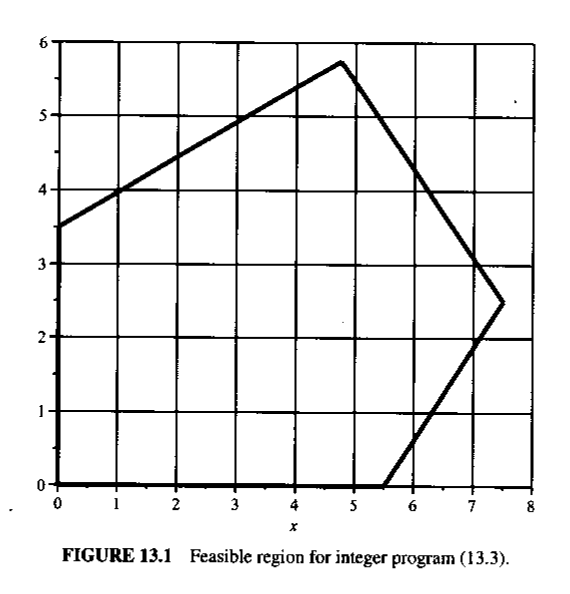
\includegraphics[width = 0.4\textwidth]{formulation_bad}
\end{multicols}

\begin{multicols}{2}

{\bf Problem B:}
\begin{align*}
      \maximize \quad & 8x + 7y \\
      \subjectto \quad & -x+2y ~\leq~ 6\\
                       & x + y ~\leq~ 10\\
                       & x - y ~\leq~ 5\\
                       & x ~\leq~ 7\\
                       & y ~\leq~ 5\\
                       & x,y \in \mathbb{Z}^{\geq 0}
\end{align*}
\vspace{6cm}

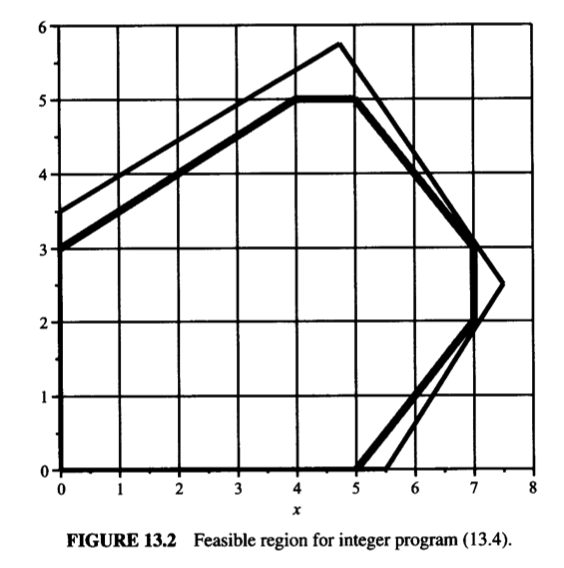
\includegraphics[width = 0.4\textwidth]{formulation_ideal}
\end{multicols}


\begin{enumerate}[(a)]
   \item On the diagrams, identify all feasible solutions to both IPs. 
   \item Are the feasible regions for problems A and B different or the same?  \wordbox
   \item What does this mean about the two problems A and B? 
   
   \answerboxone{c}{.6in}
   \item Are the LP relaxations of A and B the same?  If not, which has the higher optimal objective value?
   
   \answerboxone{c}{.5in}
\end{enumerate}
\end{problem}


\newpage

\begin{problem}
Refer back to the previous problem to answer the following:
\begin{enumerate}[(a)]
\item  Suppose an optimal solution to an IP exists.
\begin{enumerate}[i.]
\item Can an optimal solution \emph{always} be found at a corner point?  (The question from before.)

\answerboxtwo{c}{.5in}

\item Can an optimal solution \emph{sometimes} be found at a corner point?  
 
\answerboxtwo{c}{.5in}
\end{enumerate}
\item Which of the two formulations of the IP in problem 3 is easier to solve?  Why?

\answerboxone{c}{1in}

\end{enumerate}
\end{problem}

\vfill
\section{Comparing IP Formulations}


\begin{itemize}
\item Often the decision of how to formulate an IP comes down to a trade-off between quality of formulation and number of constraints:
\begin{itemize}
\item \wordbox constraints means a better (tighter) formulation, but too \catbox constraints can cause memory pressure and slow down the solver.  (More/Fewer, many/few)
\item \wordbox constraints means fewer memory problems, but results in a formulation that is not as good.  (More/Fewer)
\end{itemize}
%\item  My research has to do with developing guidelines on which constraints are the most important to include in IP formulations.
%\begin{itemize}
%\item  The idea is to get the most ``bang for your buck''.
%\end{itemize}
\end{itemize}

\bigskip
TAKEAWAY:

\begin{tcolorbox}
The way we choose to \wordbox the feasible region of an IP can have a big impact on solver performance.
\end{tcolorbox}

\vfill


\end{document}

\subsection{Better Formulation $\Rightarrow$ Better Bound}

\bigskip
If we \wordbox the integrality requirement on an integer program, it becomes a

 \wordbox program, which is (EASY or HARD) to solve.

\bigskip
Solving an LP \wordbox is a critical part of the algorithm for solving an Integer Program.

\bigskip
In general, if we are solving a \emph{maximization} IP, the solution to its \textbf{LP relaxation} provides a (LOWER or UPPER) bound on the solution to the IP.
	\begin{itemize}
		\item  A \textbf{tighter} formulation provides a \wordbox bound via its LP relaxation.
		\item  An \textbf{ideal} formulation provides an \wordbox solution via its LP relaxation!
	\end{itemize}

\begin{tcolorbox}
This idea is key for solving IPs!
\end{tcolorbox}	
\begin{problem}
Sketch a problem which proves if we're maximizing, $z_{LP} \geq z_{IP}$ and vice versa if minimizing.
\end{problem}

	

\newpage
\subsection{Convex Hull Formulation}

\begin{tcolorbox}
The \textbf{convex hull} of a set of integer feasible solutions is the \textbf{smallest convex set} that contains all of the points. 
\end{tcolorbox}

\begin{itemize}
\item Recall that a set is \textbf{convex} if the \wordbox between any two points in the set is contained in the set.  
	\begin{itemize}
	\item From SA305: if set $S$ is convex and $a \in S$ and $b \in S$, then any point of the form
	\[
	\lambda a + (1-\lambda) b 
	\] where $\lambda \in [0,1]$ is also in $S$. Graphically, this is usually illustrated as a circle vs a kidney bean.
	\end{itemize} \vspace{1in}

\item Mathematically, if $X = \{v_1,v_2,\dots,v_k\}$ is a finite set of integer points, the \textbf{convex hull} of $X$ is
\[
conv(X) = \left\{x = \sum_{i = 1}^{k} \alpha_i v_i : \sum_{i = 1}^{k} \alpha_i = 1 
\text{ and } \alpha_i \geq 0 \text{ for all } i \in \{1,~2,\dots,~k\}\right\},
\]
the set of all \wordbox \wordbox of the set $\{v_1,v_2,\dots,v_k\}$


\item Integer Program (A or B) is an example of a convex hull formulation for a set of integer feasible points.
\end{itemize}

\vfill

%%%
\newpage
\begin{problem} A formulation for a set of feasible integer solutions is pictured on the left.  The integer solutions are highlighted on the right.  Sketch the \textbf{convex hull formulation} of this set of solutions.

\vspace{0.5cm}
\begin{center}
\begin{minipage}{6.5in}
\centering
\raisebox{-0.5\height}{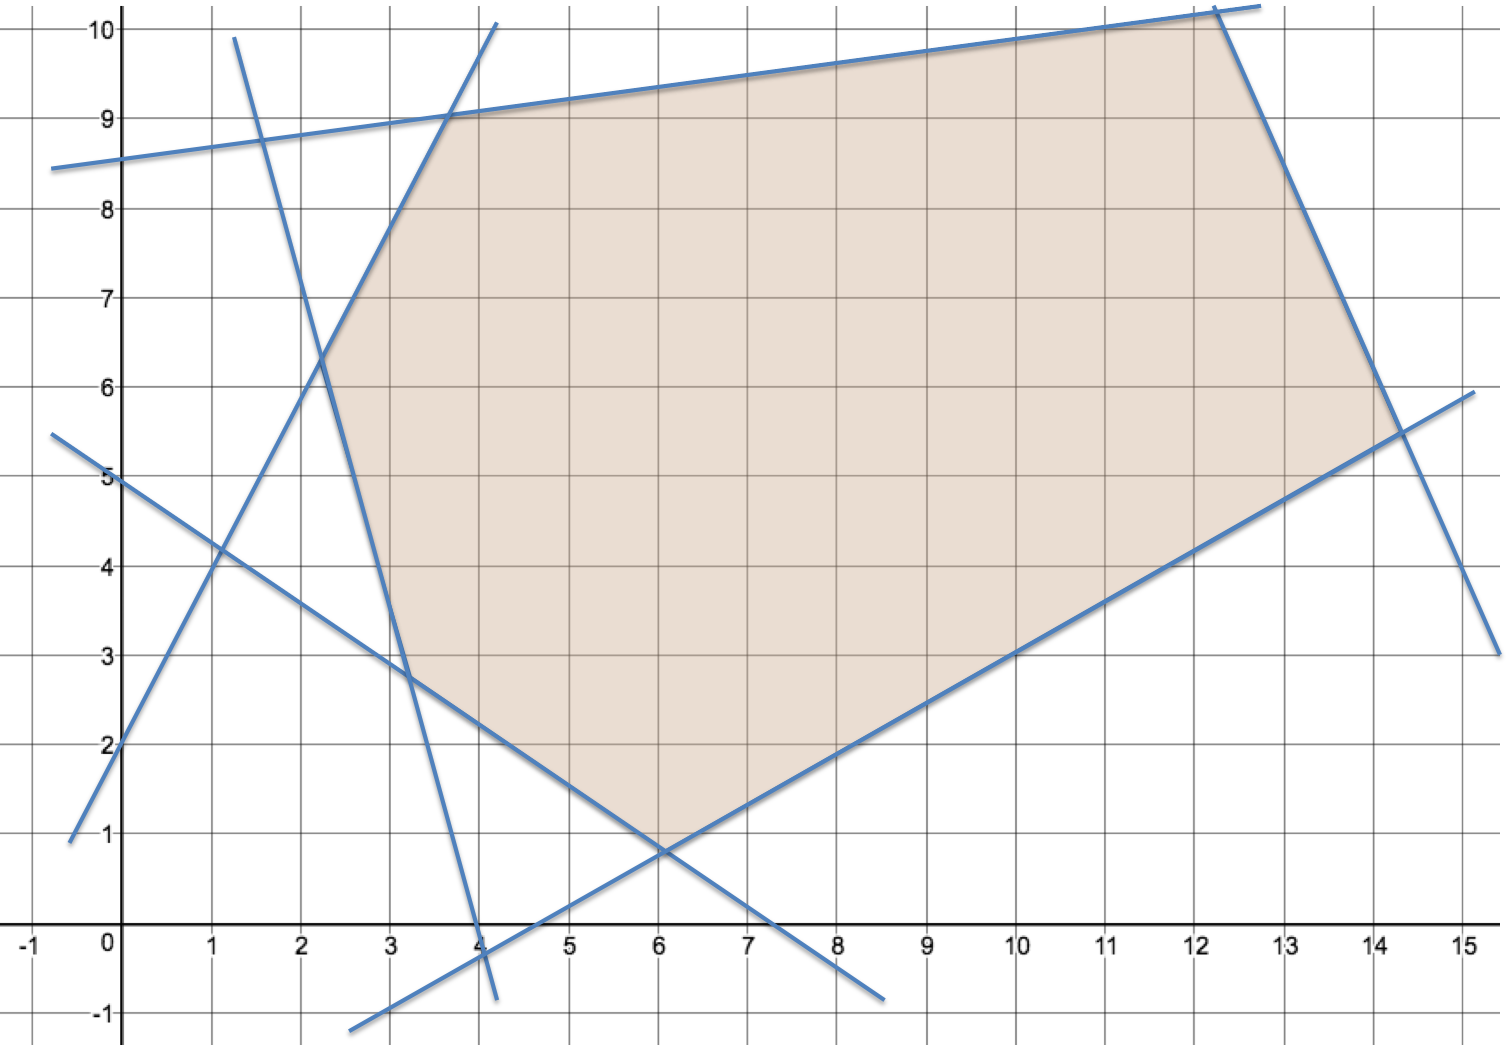
\includegraphics[width=0.35\textwidth]{convexhull_problem}}
\hspace*{0.2in}
\raisebox{-0.5\height}{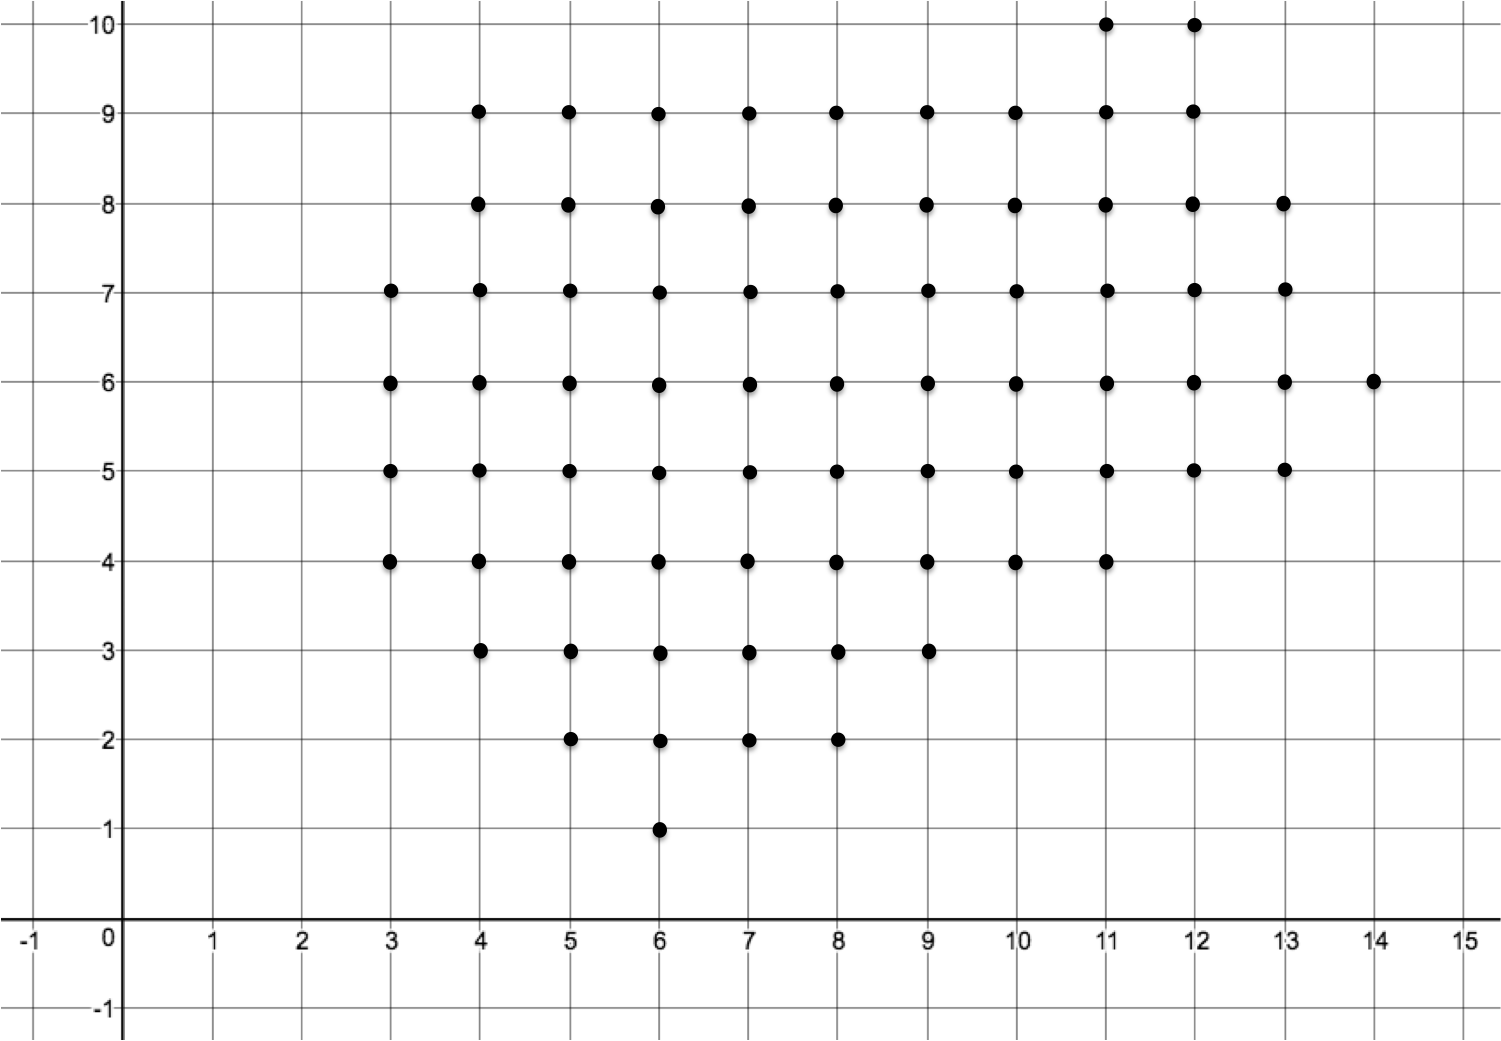
\includegraphics[width=0.6\textwidth]{convexhull_find}}
\end{minipage}
\end{center}
\end{problem}

\vfill
\begin{tcolorbox}
The \textbf{convex hull formulation} of a finite set of integer feasible solutions is considered to be the \textbf{``ideal''} formulation.
\end{tcolorbox}

Why?

\answerboxfull{c}{2cm}

\vfill
\begin{tcolorbox}
\textbf{HOWEVER, for most problems \underline{we can't use the ideal, convex hull formulation}} 

because the number of ~\wordbox~ required to describe the convex hull is often 

very, very ~\wordbox, i.e., \emph{exponential} in the number of variables.
\end{tcolorbox}

What are we to do?...
\vfill
%%%
\newpage
\section{Comparing Formulations}

\bigskip
When choosing which constraints to include in an IP formulation, there is a \textbf{tradeoff}:
\begin{itemize}
	\item use \textbf{enough} constraints to make a reasonably tight ``container'' for the feasible points,
	\item but \textbf{few enough} constraints so the resulting problem is of manageable size.
\end{itemize}

\bigskip
One strategy is to iteratively add constraints as we need them, to ~\wordbox 

\emph{fractional} solutions obtained by solving LP ~\wordbox.  We discussed this

\textbf{separation} strategy in the context of both the 

\begin{itemize}
	\item \wordbox~\wordbox~ problem, and
	\item \wordbox~\wordbox~ problems.
\end{itemize}

\subsection{Example:  Fixed-Charge Weak Vs. Strong Formulations}
Many common IP problems have been studied extensively to determine effective modeling strategies.  One such problem type is the \textbf{fixed-charge facility location problem} that we modeled earlier in the semester.  

\begin{problem}
Suppose there is a possible warehouse at location $1$ with maximum capacity $C_1$, and customers at locations $2$, $3$, and $4$.  The binary variable $z_1$ indicates whether or not facility $1$ is used.  Integer variables $x_{12}$, $x_{13}$, and $x_{14}$ represent the amount of flow on the edges leaving facility $1$.  

\begin{center}
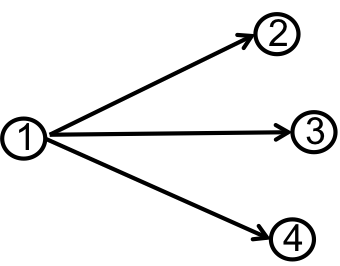
\includegraphics[width=0.2\textwidth]{facility_location}
\end{center}

We saw two different ways to enforce the requirement that if facility $1$ is closed, there is no flow out of facility $1$.

\textbf{Weak formulation:}  \hspace{3.7cm}  \textbf{Strong formulation:}

\answerbox{c}{6cm}{3cm}  \hspace{.8cm} \answerbox{c}{6cm}{3cm}

\end{problem}

\newpage

\vspace{1in}

\begin{tcolorbox}
To summarize, finding the convex hull of an integer program is the gold standard of IP formulations. That said, there are several issues with this:
	\begin{enumerate}
	\item Exponential number of constraints
	\item Potential numerical issues with tons of constraints
	\end{enumerate}
In general, we do not look for the convex hull. We do, however, use this idea to generate \textbf{cuts} when solving IPs.
\end{tcolorbox}

\newpage
(Blank for extra work)
\newpage
(Blank for extra work)

%\textbf{Fixed-Charge -- Linear Objective:}  Did you wonder why these were called the ``weak'' and ``strong'' formulations?  We compared these formulations on a very small problem.  Both formulations resulted in the same optimal solution, and both took about the same length of time.  What do you think will happen when we test these formulations on a larger problem? Why?  

%\answerboxfull{c}{2cm}

%Let's take a look at what happens when we solve a larger fixed-charge facility location problem with a \textbf{linear objective function} using \texttt{GLPK} (the \texttt{GUSEK} solver).  Record the results below.

%Weak formulation:

%\answerboxfull{c}{2cm}

%Strong formulation:

%\answerboxfull{c}{2cm}

%How can we explain this outcome?

%\answerboxfull{c}{2cm}

%The case of a linear objective function is well-studied in the context of many common problems.  This intelligence is \emph{built into most modern solvers}.

%\textbf{Fixed-Charge -- Nonlinear Objective:}   Current research focuses on \emph{nonlinear} problems.   In the presence of a \textbf{nonlinear objective function}:

%\begin{itemize}
%\item the optimal solution (IS or IS NOT) guaranteed to occur at a corner point;
%\item the \wordbox of the feasible region is more important than the boundary;
%\item we can omit constraints that don't ``cut-off'' much volume, to simplify a formulation.
%\end{itemize} 

%With a \wordbox objective function, the weak forcing constraints perform slightly better

%than the strong, due to a very similar volume and a smaller formulation.




\end{document}
